\documentclass[10pt,a4paper]{article}
\usepackage[margin=2.1cm]{geometry}
\usepackage[T1]{fontenc}
\usepackage[utf8]{inputenc}
\usepackage{mathpazo}
\usepackage[expansion=false]{microtype}
\usepackage{graphicx}
\usepackage{booktabs}
\usepackage{amsmath,amssymb}
\usepackage{tikz}
\usetikzlibrary{arrows.meta,positioning,calc,shapes.geometric,fit,backgrounds}
\usepackage{subcaption}
\usepackage{xcolor}
\usepackage{enumitem}
\usepackage{float}
\usepackage[hidelinks]{hyperref}
\usepackage{caption}
\captionsetup{font=small,labelfont=bf,width=0.95\textwidth}
\definecolor{ink}{HTML}{0B0B0B}
\definecolor{ink2}{HTML}{52514E}
\definecolor{blue1}{HTML}{2A78D6}
\definecolor{orange1}{HTML}{EB6834}
\definecolor{aqua1}{HTML}{1BAF7A}
\definecolor{yellow1}{HTML}{EDA100}
\definecolor{violet1}{HTML}{4A3AA7}
\definecolor{grey1}{HTML}{B5B3AD}
\definecolor{grey2}{HTML}{E4E3DF}
\newcommand{\code}[1]{\texttt{\small #1}}
\newcommand{\ldu}{\,LDU}
\setlist{nosep,leftmargin=1.4em}
\graphicspath{{fig/}}

\title{\vspace{-1.2cm}\textbf{Brickator: from a triangle mesh to a buildable LEGO model}\\[0.3em]
\large The volume field, the placement kernel, motifs learned from official sets, sideways building, and where the ``mechanical'' look actually comes from}
\author{\small brickator3000 --- branches \code{next} and \code{siren} --- state of the method as of 4 October 2026}
\date{}

\begin{document}
\maketitle
\vspace{-0.8cm}
\begin{abstract}
\noindent Brickator turns an arbitrary triangle mesh into a list of LEGO pieces that can actually be built: parts on the stud/plate
lattice, held by stud contact, in one connected component. The method is deliberately simple --- a fractional volume field on a
4\ldu{} grid, a lazy-greedy placement kernel that scores each part by how well its own voxelised volume explains the field, a
sequence of phases from the most constrained parts to the least, and a post-process that merges, props and braces --- and this
document describes every step with figures. It then describes the three things learnt this week by measurement rather than by
reasoning: (1)~\emph{motifs}, recurring multi-part assemblies mined from 1,148 official LDraw models, placed as compound parts in a
broad phase before any single part, including \emph{sideways} (SNOT) assemblies in all 24 axis-aligned orientations;
(2)~the vertical-pole mystery, where mirror symmetry seemed to fix something that was in fact an all-or-nothing test in the
post-process; and (3)~that the ``parasitic noise on flat surfaces'' is mostly not noise: it is the LEGO lattice being misaligned
with the model's planar faces, and a lattice fit of the scale and origin raises the chair's IoU from 0.872 to 0.922 with 9\,\%
fewer pieces. A signed-distance representation (and a SIREN fitter for the GPU) is built and measured along the way: it works,
it denoises real grain, and it only pays off once the field is quantised exactly like the part templates.
\end{abstract}

\tableofcontents

\section{Overview}
\subsection{Units and the lattice}
Everything is in LDraw units (LDU): a stud pitch is 20\ldu, a plate is 8\ldu{} tall, a brick 24\ldu{} (three plates). The engine
samples the world on a grid of $4\ldu$ --- five samples per stud in $x$ and $z$ --- and one \emph{level} per plate in $y$. A piece is
placed at integer stud cells $(i, j)$ and integer plate level $b$, with a footprint $w\times d$ studs and a height $h$ plates;
sideways pieces (Section~\ref{sec:snot}) may sit at fractions of those. LDraw's frame is $Y$-down; the engine's is $Y$-up, the two
related by $D=\mathrm{diag}(1,-1,-1)$, and every reader and writer in the code goes through that one matrix.

\begin{figure}[h]
\centering
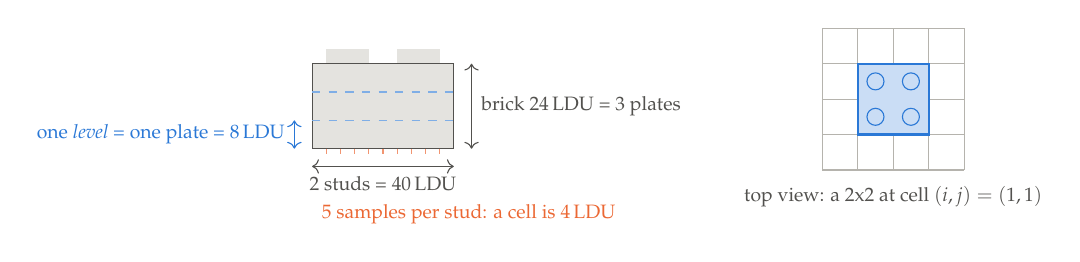
\begin{tikzpicture}[x=0.9cm,y=0.9cm,font=\scriptsize]
  % a brick 2x1 seen from the side, with the sample grid
  \fill[grey2] (0,0) rectangle (2,1.2); \fill[grey2] (0.2,1.2) rectangle (0.8,1.4); \fill[grey2] (1.2,1.2) rectangle (1.8,1.4);
  \draw[ink2] (0,0) rectangle (2,1.2);
  \draw[<->,ink2] (0,-0.25) -- (2,-0.25) node[midway,below]{2 studs = 40\ldu};
  \draw[<->,ink2] (2.25,0) -- (2.25,1.2) node[midway,right]{brick 24\ldu{} = 3 plates};
  \foreach \l in {0.4,0.8} \draw[blue1!60,dashed] (0,\l) -- (2,\l);
  \draw[<->,blue1] (-0.25,0) -- (-0.25,0.4) node[midway,left]{one \emph{level} = one plate = 8\ldu};
  \foreach \s in {0.2,0.4,...,1.8} \draw[orange1!70] (\s,0) -- (\s,-0.08);
  \node[orange1,anchor=north west] at (0,-0.65) {5 samples per stud: a cell is 4\ldu};
  % right: top view of the stud grid with a 2x2 piece
  \begin{scope}[shift={(7.2,-0.3)}]
    \foreach \i in {0,...,4} { \draw[grey1] (\i*0.5,0) -- (\i*0.5,2); \draw[grey1] (0,\i*0.5) -- (2,\i*0.5); }
    \fill[blue1!25] (0.5,0.5) rectangle (1.5,1.5); \draw[blue1,thick] (0.5,0.5) rectangle (1.5,1.5);
    \foreach \i in {0.75,1.25} \foreach \j in {0.75,1.25} \draw[blue1] (\i,\j) circle (0.12);
    \node[anchor=north,ink2] at (1,-0.1) {top view: a 2x2 at cell $(i,j)=(1,1)$};
  \end{scope}
\end{tikzpicture}
\caption{The lattice. Horizontal positions are whole studs (20\ldu), heights whole plates (8\ldu); the volume field is sampled five times
per stud and once per plate.}
\end{figure}

\subsection{The pipeline}
\begin{figure}[h]
\centering
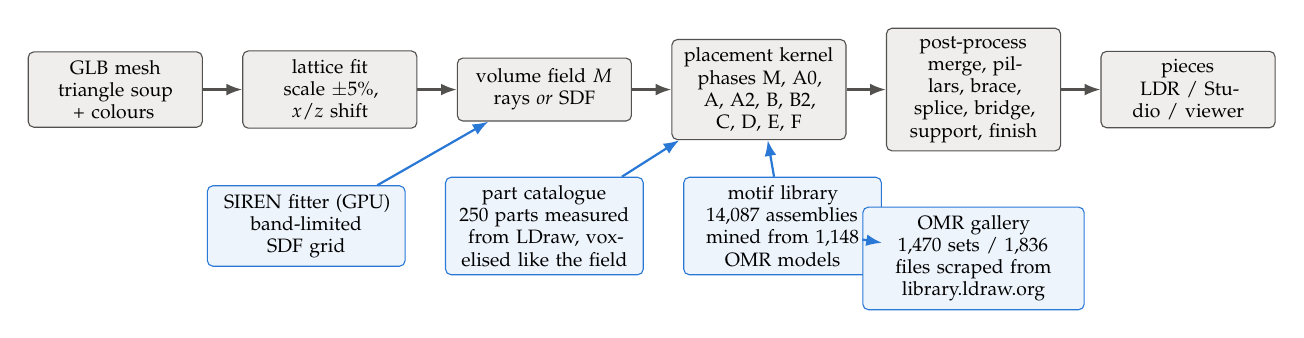
\begin{tikzpicture}[font=\scriptsize, node distance=0.35cm and 0.5cm,
  box/.style={draw=ink2, rounded corners=2pt, fill=grey2!60, minimum height=0.8cm, text width=2.0cm, align=center, inner sep=3pt},
  side/.style={draw=blue1, rounded corners=2pt, fill=blue1!8, minimum height=0.8cm, text width=2.3cm, align=center, inner sep=3pt},
  arr/.style={-{Latex[length=2mm]}, ink2, thick}]
  \node[box] (mesh) {GLB mesh\\ triangle soup + colours};
  \node[box, right=of mesh] (fit) {lattice fit\\ scale $\pm5\%$, $x/z$ shift};
  \node[box, right=of fit] (field) {volume field $M$\\ rays \emph{or} SDF};
  \node[box, right=of field] (solve) {placement kernel\\ phases M, A0, A, A2, B, B2, C, D, E, F};
  \node[box, right=of solve] (post) {post-process\\ merge, pillars, brace, splice, bridge, support, finish};
  \node[box, right=of post] (out) {pieces\\ LDR / Studio / viewer};
  \draw[arr] (mesh) -- (fit); \draw[arr] (fit) -- (field); \draw[arr] (field) -- (solve); \draw[arr] (solve) -- (post); \draw[arr] (post) -- (out);
  \node[side, below=0.7cm of field] (cat) {part catalogue\\ 250 parts measured from LDraw, voxelised like the field};
  \node[side, right=of cat] (mot) {motif library\\ 14,087 assemblies mined from 1,148 OMR models};
  \node[side, left=of cat] (siren) {SIREN fitter (GPU)\\ band-limited SDF grid};
  \draw[arr, blue1] (cat) -- (solve); \draw[arr, blue1] (mot) -- (solve); \draw[arr, blue1] (siren) -- (field);
  \node[side, below=0.7cm of post, text width=2.6cm] (ldraw) {OMR gallery\\ 1,470 sets / 1,836 files scraped from library.ldraw.org};
  \draw[arr, blue1] (ldraw) -- (mot);
\end{tikzpicture}
\caption{The pipeline. Grey: the per-model path. Blue: what is prepared once --- the catalogue, the motif library mined from official
sets, and (optionally) a field fitted on the GPU.}
\end{figure}

The per-model path is \code{pipeline.setup} (mesh, samples, symmetry, field) $\to$ \code{scoreJob} over a few grid phases $\to$
\code{finishJob} on the best one (colours, merges, connectivity, finish). Everything is pure JavaScript (\code{claude/app/src/brickgen}),
runs in Node or a web worker, and the dev panel in \code{StudioApp} exposes every option named in this document.

\section{The volume field}
\subsection{Vertical rays}
The field $M[\ell][z][x]\in[0,1]$ is the fraction of each 4\ldu$\times$8\ldu$\times$4\ldu{} cell that is inside the model. It is
built from vertical rays: one ray per $(x,z)$ sample column, every triangle it crosses recorded with its height and facing
(\code{grid.columnHits}), then the hits of a column paired in order --- enter, exit, enter, exit --- the even--odd rule, so that the
air between a biplane's wings, or inside a bowl, stays air (\code{spansVolume}, mode \code{hollow}). Each solid interval is cut
into plate levels, and a level's fill is the exact fraction of the plate the interval covers. Three small rules follow:
air thinner than \code{minGap} (6\ldu) between two intervals is closed; the first interval snaps to the ground when it is within
\code{snap} (12\ldu) of it; and a sheet thinner than 0.8 plate is fattened to one plate (\code{minThick}), so a single-sided wing
does not vanish.

\begin{figure}[h]
\centering
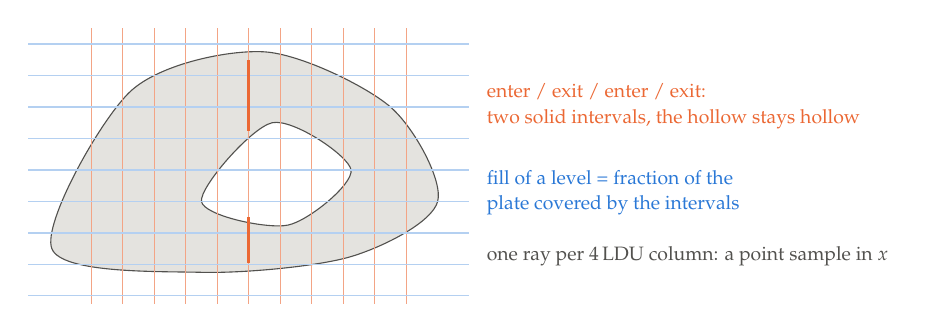
\begin{tikzpicture}[x=1cm,y=1cm,font=\scriptsize]
  % section of a shape with rays
  \fill[grey2] plot[smooth cycle] coordinates {(0.5,0.6) (1.5,2.6) (3.2,3.1) (4.8,2.4) (5.4,1.2) (4.3,0.5) (2.4,0.3)};
  \fill[white] plot[smooth cycle] coordinates {(2.4,1.2) (3.3,2.2) (4.3,1.6) (3.5,0.9)};
  \draw[ink2] plot[smooth cycle] coordinates {(0.5,0.6) (1.5,2.6) (3.2,3.1) (4.8,2.4) (5.4,1.2) (4.3,0.5) (2.4,0.3)};
  \draw[ink2] plot[smooth cycle] coordinates {(2.4,1.2) (3.3,2.2) (4.3,1.6) (3.5,0.9)};
  \foreach \x in {1.0,1.4,...,5.0} \draw[orange1!60] (\x,-0.1) -- (\x,3.4);
  \foreach \l in {0,0.4,...,3.2} \draw[blue1!35] (0.2,\l) -- (5.8,\l);
  \draw[orange1,very thick] (3.0,0.42) -- (3.0,1.0); \draw[orange1,very thick] (3.0,2.1) -- (3.0,3.0);
  \node[orange1,anchor=west] at (5.9,2.6) {enter / exit / enter / exit:};
  \node[orange1,anchor=west] at (5.9,2.25) {two solid intervals, the hollow stays hollow};
  \node[blue1,anchor=west] at (5.9,1.5) {fill of a level = fraction of the};
  \node[blue1,anchor=west] at (5.9,1.15) {plate covered by the intervals};
  \node[ink2,anchor=west] at (5.9,0.5) {one ray per 4\ldu{} column: a point sample in $x$};
\end{tikzpicture}
\caption{The ray field. Exact along $y$, point-sampled along $x$ and $z$ --- the asymmetry that Section~\ref{sec:lattice} and
Section~\ref{sec:sdf} both come back to.}
\end{figure}

\begin{figure}[h]
\centering
\includegraphics[width=0.98\textwidth]{field_slices}
\caption{Four plate levels of the duck's field at 24 studs (colour = fill). The crust option has already hollowed the body: only a
40\ldu{} shell is kept, so the solver fills a wall, not a block.}
\end{figure}

\subsection{Crust, islands, points}
After the cast, \code{carveCrust} erases every solid cell deeper than 40\ldu{} from air (a bucketed Dijkstra with 4\ldu{} steps
sideways and 8\ldu{} up/down), so that the model becomes a shell and the part count stays sane; \code{islands.js} either connects
floating components with a minimum-spanning tree of thin tubes or decimates floaters below a size. The 200k area-weighted surface
samples that drive colouring are also splatted into a point count $P$ per cell, which the thin-feature phase uses to find
features the rays missed. Mirror symmetry, when detected in the samples, shifts the model so the plane lies on a stud boundary,
averages the field with its mirror and places each piece with a twin --- Section~\ref{sec:poles} has what that really does.

\section{The lattice: where the ``parasitic noise'' comes from}\label{sec:lattice}
The observation that started the \code{siren} branch: flat-ish surfaces come out as a mosaic of small plates, as if the mesh were
noisy. To separate the mesh from the method, \code{test/noise\_bench.mjs} builds a watertight synthetic house (12$\times$8 studs,
6-brick walls, a 45$^\circ$ gable roof, faces subdivided to 6\ldu{}), displaces its vertices along their normals with Gaussian
grain of $\sigma=0,1,2,4\ldu$, solves, and grades the result against the field of the \emph{clean} house \emph{in the same
frame}. Both italics were bugs in the first versions of the bench: grading against the noisy field grades the grain as truth, and
the noisy bounding box moves the normalisation, which alone costs 0.4 of mean field error.

\begin{figure}[h]
\centering
\begin{subfigure}{0.49\textwidth}\centering\includegraphics[width=\textwidth]{r_house_clean_src}\caption{the clean house}\end{subfigure}
\begin{subfigure}{0.49\textwidth}\centering\includegraphics[width=\textwidth]{r_house_noisy_rays_src}\caption{grain $\sigma=2\ldu$ (a plate is 8)}\end{subfigure}
\caption{The test geometry. The grain is a quarter of a plate --- invisible at LEGO scale, but a quarter of a cell.}
\end{figure}

\begin{figure}[h]
\centering
\includegraphics[width=\textwidth]{house_fields}
\caption{A vertical slice through the field at mid-$x$ in four situations (levels up, $z$ across). Grain alone (second) breaks the
walls into partial cells and the solver into 413 pieces; snapping the frame to the lattice (third) brings it back to 208 with the
very same rays; the filtered SDF (fourth) cleans the remaining speckle.}
\end{figure}

\begin{figure}[h]
\centering
\includegraphics[width=0.9\textwidth]{phases}
\caption{Where the pieces come from. On the clean house the fill (B) and skin (A) phases do the work. Under grain the big parts fail the
error budget and 300 of 486 pieces come from the mop-up phases \emph{relaxed} and \emph{thin}; the lattice fit returns the work to
fill and skin.}
\end{figure}

\begin{figure}[h]
\centering
\includegraphics[width=0.98\textwidth]{noise_bench}
\caption{The controlled experiment (merged pieces, and IoU against the clean field in the same frame). One LDU of grain doubles the
piece count with plain rays. The lattice fit recovers most of it; the median-filtered SDF on top reaches the clean mesh's own numbers
(at $\sigma=4$: 145 pieces / 0.859 vs 145 / 0.861 for the clean mesh in that frame).}
\end{figure}

\subsection{Why one LDU matters}
The fill phase accepts a part only if the $L_1$ residual between the part's volume and the field is below \code{max\_err}
$=0.06$ of the part's box (Section~\ref{sec:kernel}). A 2$\times$4 plate has 200 samples; $\pm1\ldu$ of grain is $\pm0.12$ of fill
per sample on the top level, so the residual exceeds the budget with no shape error at all. Worse, the grain moves mass across a
plate boundary: the level below becomes 90\,\% full and the level above 10\,\%, and neither is fillable. The same thing happens
without any grain when a flat face sits at a fractional plate height --- and it does for every real model, because the scale is set
by ``longest side $= N$ studs'' from the bounding box, which is a beak or a tail, not the planes. Translating the \emph{clean}
house by 1--4\ldu{} costs it +60\,\% pieces and 6 IoU points.

\subsection{The lattice fit}
\code{grid.latticeFit} looks at the planar faces before anything is voxelised. For each axis, the faces whose normal is within
25$^\circ$ of it give positions $p_f$ with areas $a_f$; the score of a scale $s$ is the circular resultant
\[
R_{\mathrm{axis}}(s)=\frac{\bigl|\sum_f a_f\,e^{2\pi i\, s\,p_f/\mathrm{period}}\bigr|}{\sum_f a_f},
\]
which is 1 when every face is lattice-consistent and about 0 for random positions (period = stud for $x,z$; for $y$ the ground
anchors the phase, so the real part is used with period = plate). A 1-D search over $s\in[1-\mathrm{tol},1+\mathrm{tol}]$ of the
bounding-box scale maximises $R_x+R_y+R_z$; the shift per axis is the phase of the resultant, taken as the smallest move onto a
boundary. A model with no planar faces scores $\approx0.3$ everywhere and would be rescaled on noise, so the scale only moves
when the score gains at least \code{alignMinGain} $=0.15$; the shifts always apply. The whole-cell phase search the engine already
had (\code{offsets}) is then a refinement.

\begin{figure}[h]
\centering
\begin{subfigure}{0.46\textwidth}\centering\includegraphics[width=\textwidth]{lattice_curve}\caption{the score over scale for the noisy house}\end{subfigure}\hfill
\begin{subfigure}{0.52\textwidth}\centering\includegraphics[width=\textwidth]{results_align}\caption{on the real models, full options}\end{subfigure}
\caption{The lattice fit. It costs nothing (a histogram and a 1-D search) and is the only change this week that helps every man-made
model: chair $0.872\to0.922$ with 9\,\% fewer pieces, table $0.690\to0.789$. The biplane has no planes; it keeps its scale and loses
1.5 points to a shift made on weak evidence.}
\end{figure}

\section{The placement kernel}\label{sec:kernel}
\subsection{Part templates}
Every catalogue part is voxelised \emph{exactly like the field}: from the part's measured height profile (\code{top}/\code{bot}
per sample, or a per-level \code{cover} for shells) the exact span fraction per plate in $y$, a point sample per cell in $x$ and
$z$ (\code{variants.baseVolume}). The 250 parts come from the LDraw library through \code{claude/generator}: analytic boxes for
bricks, plates and tiles; measured volumes for slopes, curves, cheese slopes, inverted slopes, rounds, wedges, arches, panels and
dishes. Each part has its stud cells, its kind, and four yaw rotations (duplicates merged).

\begin{figure}[h]
\centering
\includegraphics[width=\textwidth]{templates}\\[2pt]
\begin{subfigure}{0.19\textwidth}\centering\includegraphics[width=\textwidth]{r_part_3039}\caption*{3039 slope 2x2}\end{subfigure}
\begin{subfigure}{0.19\textwidth}\centering\includegraphics[width=\textwidth]{r_part_54200}\caption*{54200 cheese}\end{subfigure}
\begin{subfigure}{0.19\textwidth}\centering\includegraphics[width=\textwidth]{r_part_3062b}\caption*{3062b round 1x1}\end{subfigure}
\begin{subfigure}{0.19\textwidth}\centering\includegraphics[width=\textwidth]{r_part_3665}\caption*{3665 inverted}\end{subfigure}
\begin{subfigure}{0.19\textwidth}\centering\includegraphics[width=\textwidth]{r_part_3040}\caption*{3040 slope 2x1}\end{subfigure}
\caption{Part templates. Top: the voxelised volume $V$ of three parts, level by level. The slope's face is a ramp of fractional fills; the
cheese slope is two levels of it; the round brick's disc leaves its corner samples empty. Bottom: the parts themselves.}
\end{figure}

\subsection{Scoring}
A candidate is a part variant $v$ at a lattice pose $(b,j,i)$. Over the samples of its box, with $V$ the template and $M$ the
field that is \emph{still unexplained} (the solver subtracts what it places),
\[
\mathrm{ov}=\sum \min(M,V),\qquad \mathrm{over}=\sum |V-M|,\qquad
\mathrm{net}=\mathrm{ov}-w_{\mathrm{err}}\,\mathrm{over}-\mathrm{piece\_pen}\cdot n_{\mathrm{pieces}}+\mathrm{bonus}(\mathrm{kind}).
\]
A candidate is admissible when $\mathrm{ov}/|V|\ge$ \code{min\_cov} and $\mathrm{over}/\mathrm{box}\le$ \code{max\_err}, both
per phase; a tile is admissible only where the level above is exposed; a candidate colliding with what is placed is dropped. The
phase takes candidates from a heap by net score, re-checks each at pop time (the field has changed), places it, and repeats
(\code{Solver.runPhase}, lazy greedy).

\begin{figure}[h]
\centering
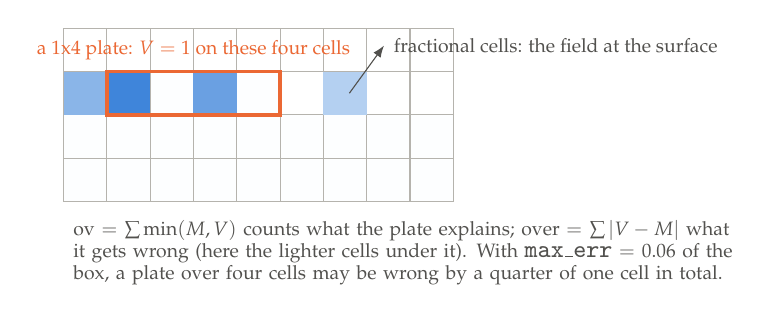
\begin{tikzpicture}[x=0.55cm,y=0.55cm,font=\scriptsize]
  \foreach \x in {0,...,8} \foreach \y in {0,...,3} { \pgfmathsetmacro{\f}{ (\y<2) ? 1 : ((\y==2) ? (\x<5 ? 0.9 : 0.15) : 0) } \fill[blue1!\f!white, draw=grey1] (\x,\y) rectangle (\x+1,\y+1); }
  \fill[blue1!55] (0,2) rectangle (1,3); \fill[blue1!90] (1,2) rectangle (2,3); \fill[blue1!70] (3,2) rectangle (4,3); \fill[blue1!35] (6,2) rectangle (7,3);
  \draw[orange1, very thick] (1,2) rectangle (5,3);
  \node[orange1, anchor=south] at (3,3.05) {a 1x4 plate: $V=1$ on these four cells};
  \draw[ink2,-{Latex[length=1.5mm]}] (6.6,2.5) -- (7.4,3.6) node[anchor=west,ink2] {fractional cells: the field at the surface};
  \node[anchor=north west, ink2, text width=8.5cm] at (0,-0.2) {ov $=\sum\min(M,V)$ counts what the plate explains; over $=\sum|V-M|$ what it gets wrong (here the lighter cells under it). With \code{max\_err} $=0.06$ of the box, a plate over four cells may be wrong by a quarter of one cell in total.};
\end{tikzpicture}
\caption{The score, on one level. The field $M$ is shown as blue intensity; the solver places the part whose template best explains the
cells it covers, and then removes that volume from $M$.}
\end{figure}

\paragraph{The prefilter.} Scoring every variant at every pose would be hopeless, so \code{candidates()} first reads a
cell-level integral image of $M$: the box sum $S$ of a pose costs eight lookups, and $S\ge$ \code{min\_cov}$\cdot|V|$ and
$|S-|V||\le$ \code{max\_err}$\cdot$box are necessary conditions. Solid boxes (bricks, plates, tiles) need nothing more, because
for $V\equiv1$ both sums reduce to the box sum. Shaped parts go through a per-level bound next and the exact sample loop last.

\paragraph{beatFlat.} A shaped part only wins where it explains the box better than the best stack of flat parts would
(\code{beatFlat} $=0.9$: its error must be below 90\,\% of the flat stack's). Without it the skin phase paved every surface with
stud-less 1$\times$1 curved parts --- the first bug found in this project, and the one that defined its scoring.

\subsection{Phases}
\begin{table}[H]
\centering\small
\begin{tabular}{p{1.7cm}p{4.2cm}p{9.6cm}}
\toprule
phase & parts & role, tolerances \\
\midrule
M-motif & compound assemblies & the broad phase, Section~\ref{sec:motifs}; \code{min\_cov} .85, \code{max\_err} .06, per-part penalty, beatFlat .8 \\
A0-round & round bricks / plates & \code{max\_err} .12, bonus .4 --- pillars and bosses before anything flat \\
A-skin, A2 & slopes, curves, cheese, inverted; then the extended shapes & the surface; \code{min\_cov} .65, \code{max\_err} .14, kind bonuses \\
B-fill, B2 & bricks, plates, shaped boxes (and technic bricks) & the body; \code{max\_err} .06 then .16 \\
C-relaxed & 1-plate parts & \code{max\_err} .5, small penalty: the mop-up of the surface \\
D-fallback & 1x1 plates & every cell still $\ge$ \code{fallbackMin} \\
E-thin & 1x1 plates near surface points & features thinner than a cell, from the point splat $P$ \\
F-tube & & the MST tubes of \code{islands} \\
\bottomrule
\end{tabular}
\caption{The phase schedule: from the most constrained parts to the least. The phase a piece came from is kept on the piece, which is how
Figure~5 was made.}
\end{table}

\subsection{Grid phases and symmetry}
The lattice can sit at several whole-cell offsets relative to the model; the engine casts once on a padded grid and solves a few
windows of it (\code{offsets}, multiples of 4\ldu{} up to the \emph{precision} setting), keeping the one with the best
$\mathrm{IoU}-0.002\cdot\mathrm{pieces}$. With the lattice fit of Section~\ref{sec:lattice} this is a refinement; before it, it
was the only alignment there was.

\section{Post-processing}\label{sec:post}
The solver's pieces are then merged (three stacked plates of one footprint into a brick, neighbouring plates into one, a re-tile of
stacked plates of any footprint into bricks), the exposed stud-less skin is turned into tiles where a tile would be seen, and
connectivity is repaired: \code{bracing} adds plates between components that nearly touch, \code{splice} and \code{bridge} add
chains of plates back to a seed, \code{supports} drops columns to the ground, all under a stud-contact union-find in which a
piece holds another only through studs. A motif placed as one assembly is one component by construction (\code{mi}), and a
sideways assembly is rigid: no merge pass may touch any of its pieces (Section~\ref{sec:snot}).

\subsection{Pillars, and what mirror symmetry was really doing}\label{sec:poles}
\code{pillars()} turns a free-standing column of 1$\times$1 pieces into round bricks. The user reported that with mirror symmetry
\emph{on} a biplane's struts came out as clean orange stacks, and with it \emph{off} as ``inconsistent, poorly evaluated and
incomplete stacks''. Symmetry does three separable things, so the first step was to split them (\code{symField},
\code{symTwins}) and measure on be2 at 48 studs:

\begin{center}\small
\begin{tabular}{lcccc}\toprule
 & pieces & IoU & components & clean poles \\ \midrule
symmetry off & 735 & 0.400 & 4 & 6 of 14 \\
all three & 787 & 0.369 & 3 & 8 of 12 \\
A: sub-stud shift only & 721 & 0.399 & 6 & 6 of 16 \\
B: field averaging only & \textbf{701} & \textbf{0.397} & \textbf{1} & \textbf{9 of 15} \\
C: mirror twins only & 827 & 0.365 & 1 & 4 of 17 \\ \bottomrule
\end{tabular}
\end{center}

The benefit was the field averaging, and two hypotheses for why --- aliasing of the point-sampled field (tested with ray
supersampling: no), lateral smoothing (tested: helps aircraft, hurts dense models) --- were both wrong. The actual cause was
in \code{pillars} itself: a column became round bricks only if the ring of eight cells around it was empty \emph{at every level
of the run}, and one stray neighbour at one level rejected the whole column. Instrumenting the test on be2: of 56 candidate
columns, 52 were rejected, all 52 by the ring, many of them 8--16 levels tall and blocked at a single level. Mirroring the field had
merely tidied those neighbourhoods up. Two unconditional changes --- split a run at its blocked levels and convert each clear
stretch; let an adjacent 1$\times$1 column (a strut pair, a railing) not count as a wall (\code{pillarCluster} $=2$) --- raised
pole completion with symmetry off from 49\,\% to 83\,\%, IoU unchanged everywhere, pieces +2.6\,\% at worst.

\begin{figure}[h]
\centering
\begin{subfigure}{0.49\textwidth}\centering\includegraphics[width=\textwidth]{r_poles_old}\caption{ring veto: 4 round pieces}\end{subfigure}
\begin{subfigure}{0.49\textwidth}\centering\includegraphics[width=\textwidth]{r_poles_new}\caption{split + thin neighbours: 124 round pieces}\end{subfigure}
\includegraphics[width=0.8\textwidth]{poles_numbers}
\caption{The biplane's struts (orange = round bricks), with the old and the new rule, symmetry off, lattice-fitted frame.}
\end{figure}

\section{Learning from official sets: motifs}\label{sec:motifs}
\subsection{Why}
The greedy kernel chooses one part at a time by local fit, so its layouts are ``mechanical'': a tiling that never looks like a set
designer's work. Official sets, as LDraw files, show which combinations represent a rounded edge, a roof ridge, a pillar, a hull, and
which recur set after set. The idea: mine those recurring assemblies and let the solver place a whole assembly at once, before any
single part --- a broad phase --- and let the existing phases fill what is left.

\subsection{The dataset}
There was no list of the LDraw Official Model Repository's files, so one was built by scraping the site: 1,470 sets, 1,836 model
files (\code{docs/omr/index.json}); 1,148 of the models on disk are usable (Technic-only batches excluded). Rebrickable's MOCs are
behind a bot check and were left out; the HuggingFace dump \code{DylanRiden/sets\_lego\_omr\_full} is a subset of this (1,367 sets)
with theme and year metadata.

\begin{figure}[h]
\centering
\includegraphics[width=\textwidth]{dataset}
\caption{The OMR gallery. Left: parts per model. Middle: the parts people use most --- plates, 1$\times$1 rounds, tiles. Right: how much
of it the engine can express, by placement: 43.5\,\% upright on the lattice (a third of that through a ``bulk alias'' that maps a
decorated part to its plain shape), 5.7\,\% sideways on the 4\ldu{} grid, and a third in parts the catalogue does not have.}
\end{figure}

\begin{figure}[h]
\centering
\begin{subfigure}{0.49\textwidth}\centering\includegraphics[width=\textwidth]{r_omr_10158}\caption{10158}\end{subfigure}
\begin{subfigure}{0.49\textwidth}\centering\includegraphics[width=\textwidth]{r_omr_10013}\caption{10013}\end{subfigure}
\caption{Two OMR models, rendered from their MPD files by the paper's own LDraw reader.}
\end{figure}

\subsection{From an LDraw file to engine pieces}
\code{motifs/ldraw.js} reads MPD sections, sub-models and aliases; \code{placements.js} is the exact inverse of the engine's LDR
writer: a placement whose rotation is one of the 24 axis-aligned orientations and whose box corner sits on the lattice (whole
studs and plates upright; fifths of a stud and half plates sideways) becomes an engine piece. Part ids are resolved exactly, by
mould family, or by bulk equivalence read from the description and verified against the bounding box. Everything else becomes an
``unknown'' box. A round trip --- pieces $\to$ LDR $\to$ reader $\to$ pieces --- is a test: 1,355 pieces of a generated duck, 61
of them sideways, come back with 0 differences, and 288 of 288 part$\times$orientation cases.

\subsection{Mining}
A motif is the content of a window $W\times D\times H$ (studs, studs, plates) that no piece crosses, that touches no unknown cell,
that holds at least two pieces and 40\,\% fill, and that is tight (a piece touches each of its six faces). Every window of 81
footprints $\{1,2,3,4,5,6,8,10,12\}^2$ and heights up to 12 (at most 512 cells) is tested with prefix sums of ``a piece straddles /
starts / ends on this plane here'', so a model costs about a second. Pieces at half-stud offsets form their own parity class. The
key of a window is the sorted list of (part, orientation, offset), canonical over the four yaws; counts and the number of distinct
source models are kept per key.

\begin{figure}[h]
\centering
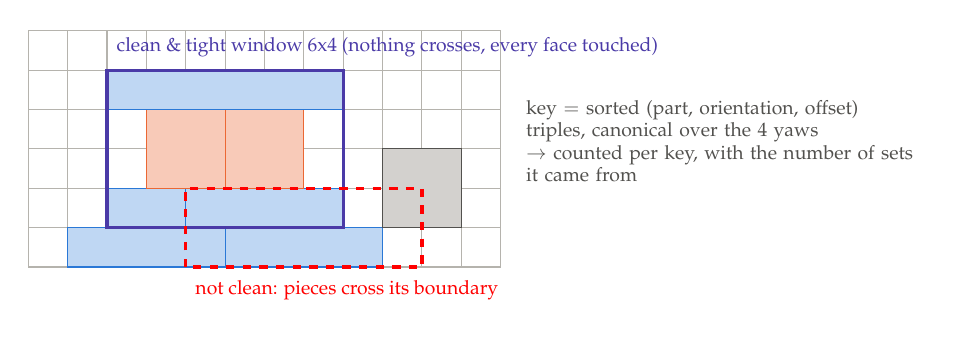
\begin{tikzpicture}[x=0.5cm,y=0.5cm,font=\scriptsize]
  \foreach \x in {0,...,12} \draw[grey1] (\x,0) -- (\x,6); \foreach \y in {0,...,6} \draw[grey1] (0,\y) -- (12,\y);
  % pieces: rectangles
  \fill[blue1!30,draw=blue1] (1,0) rectangle (5,1); \fill[blue1!30,draw=blue1] (5,0) rectangle (9,1);
  \fill[blue1!30,draw=blue1] (2,1) rectangle (4,2); \fill[blue1!30,draw=blue1] (4,1) rectangle (8,2);
  \fill[orange1!35,draw=orange1] (3,2) rectangle (5,4); \fill[orange1!35,draw=orange1] (5,2) rectangle (7,4);
  \fill[blue1!30,draw=blue1] (2,4) rectangle (8,5); \fill[grey1!60,draw=ink2] (9,1) rectangle (11,3);
  \draw[violet1, very thick] (2,1) rectangle (8,5);
  \node[violet1, anchor=south west] at (2,5.1) {clean \& tight window 6x4 (nothing crosses, every face touched)};
  \draw[red, very thick, dashed] (4,0) rectangle (10,2);
  \node[red, anchor=north west] at (4,-0.1) {not clean: pieces cross its boundary};
  \node[anchor=west, ink2, text width=5cm] at (12.4,3.2) {key $=$ sorted (part, orientation, offset) triples, canonical over the 4 yaws \\ $\to$ counted per key, with the number of sets it came from};
\end{tikzpicture}
\caption{Mining windows on a side view of a model (orange: two slopes, blue: plates, grey: an unknown part). The violet window is a
motif candidate; the red one is not.}
\end{figure}

Over 978 models with enough expressible pieces: 168,925 grid pieces, 897,574 clean windows, 46,611 distinct assemblies, 14,087
motifs kept (seen at least twice), 789 of them with a sideways part.

\begin{figure}[h]
\centering
\includegraphics[width=0.9\textwidth]{motif_stats}
\caption{The library. Most motifs are 2--4 parts; the occurrence counts are Zipf-like, a few hundred assemblies account for most of
what is seen.}
\end{figure}

\subsection{The library in the solver}
Every kept motif becomes a \emph{compound variant}: the same object the solver's part variants are (a rasterised volume $V$, a
footprint, a height, per-level sums), plus its parts and a bonus $\mathrm{motifBonus}+\mathrm{motifBonusLog}\cdot\log_2(\mathrm{models})$.
The kernel scores it unchanged; only \code{\_place} learned to expand it into its real pieces, all tagged with the motif and an
assembly id. Solid boxes (pure brick/plate stacks) are dropped --- one part already does that job --- and so are plate-only
arrangements and rows of 1$\times$1 rounds, which took the skin before the slope phase ran. The $x$-mirror of every motif whose
parts have a mirror twin is added. 1,174 motifs give 5,316 variants in the live library (286 sideways).

\begin{figure}[h]
\centering
\foreach \k in {0,...,5} {\begin{subfigure}{0.158\textwidth}\centering\includegraphics[width=\textwidth]{r_motif_\k}\end{subfigure}\hfill}\\[2pt]
\foreach \k in {6,...,11} {\begin{subfigure}{0.158\textwidth}\centering\includegraphics[width=\textwidth]{r_motif_\k}\end{subfigure}\hfill}
\caption{Twelve of the most frequent shaped motifs (one per distinct part set): cheese-slope rows and pairs, roof ridges, inverted-slope
pairs, wall-with-slope, round-brick pillars, corner frames.}
\end{figure}

\subsection{What the tuning taught}
Three findings, all now defaults: a motif must pay the per-part penalty for \emph{each} of its parts, else two-part motifs beat every
single part; no brick/plate-only motifs; and \code{beatFlat} applies to motifs too, because the broad phase runs before any brick
and a big motif with 10\,\% shape error used to win by sheer size. Skipping motifs while the grid phases are scored was a 10$\times$
speed-up. Two things measured and kept off: offering the 45 newly measured shape parts (arches, panels, dishes, corner tiles)
as solo candidates (6--15\,\% more pieces at the same IoU, so they are motif-only), and stretching periodic motifs to lengths the
sets did not contain (components 1 $\to$ 25--57: a stretched motif is a plausible shape that was never a real assembly).

\begin{figure}[h]
\centering
\includegraphics[width=\textwidth]{motif_results}
\caption{Motifs off, on without sideways assemblies, on with them (24 studs, extended part set). Recall rises on every model that uses
them; IoU rises on three of five; the price is pieces, because an assembly is several parts where one big brick would do.}
\end{figure}

\section{Sideways building (SNOT)}\label{sec:snot}
In the OMR, 23\,\% of catalogue parts are placed non-upright, a third of those at exact quarter turns: plates, tiles and cheese
slopes used as side panels on headlight bricks, side-stud bricks and brackets. A sideways sub-assembly \emph{and the connector that
holds it} is one compound motif, and the engine needed to say it.

\begin{figure}[h]
\centering
\begin{subfigure}{0.24\textwidth}\centering\includegraphics[width=\textwidth]{r_part_4070}\caption*{4070 headlight}\end{subfigure}
\begin{subfigure}{0.24\textwidth}\centering\includegraphics[width=\textwidth]{r_part_87087}\caption*{87087 stud on side}\end{subfigure}
\begin{subfigure}{0.24\textwidth}\centering\includegraphics[width=\textwidth]{r_part_11211}\caption*{11211 two studs on side}\end{subfigure}
\begin{subfigure}{0.24\textwidth}\centering\includegraphics[width=\textwidth]{r_part_44728}\caption*{44728 bracket}\end{subfigure}
\caption{The hosts: parts with studs on a vertical face.}
\end{figure}

\code{motifs/orient.js} is the centre: the 24 axis-aligned orientations as matrices (0--3 the plain yaws), the part as 4\ldu{} cubes
from its cover or its profiles, and \code{orientPart} giving the turned volume with its box origin and the LDraw matrix. Because
4\ldu{} divides both the stud (20) and the plate (8), a turned part fits the existing field; the library rasterises a motif in
4\ldu{} slices along $y$ and only collapses to plate levels at the end, since 44\,\% of the OMR's sideways parts start half a level
up. The reader, the rasteriser and the writer share that one module, so they agree by construction.

Three invariants were needed before SNOT paid off, each found by a measurement:
\begin{enumerate}
\item \textbf{A sideways motif must carry its own host.} A mining window can clip out the headlight brick whose side studs hold the
part; the remainder cannot be built, and the stud-contact test reports it as a floating component (35 of 38 extra components on the
duck were exactly that). A sideways motif is kept only when one of its upright parts offers side studs, recognised from the LDraw
description.
\item \textbf{A sideways assembly is rigid.} The side studs that carry a part belong to another piece of the same assembly;
merging that piece away cuts the part loose. One predicate, \code{post.free(p)}, now guards every merge, re-cut and flatten pass
--- the last leak was \code{mergePairs} filtering the partner of a pair but not the first piece.
\item \textbf{The repair passes treat a sideways piece as occupancy only.} It has no top face at a plate boundary and sits at a
fractional level, so it can never anchor a brace; before that guard, post-processing emitted upright plates at $b=5.5$.
\end{enumerate}
A fourth thing the connectors exposed: \code{vertical()} chose the brick for a three-plate merge with a last-wins map over the
catalogue, and the connectors, appended last, won the 1$\times$1, 1$\times$2 and 1$\times$4 keys --- every such merge became a
side-stud brick holding nothing. Footprint lookups now only see plain boxes.

\begin{figure}[h]
\centering
\foreach \k in {0,...,3} {\begin{subfigure}{0.24\textwidth}\centering\includegraphics[width=\textwidth]{r_snot_\k}\end{subfigure}\hfill}\\[2pt]
\foreach \k in {4,...,7} {\begin{subfigure}{0.24\textwidth}\centering\includegraphics[width=\textwidth]{r_snot_\k}\end{subfigure}\hfill}
\caption{Eight of the most frequent sideways motifs (cyan = the sideways part): tiles and plates on headlight bricks, side-stud bricks
and brackets.}
\end{figure}

\begin{figure}[h]
\centering
\begin{subfigure}{0.49\textwidth}\centering\includegraphics[width=\textwidth]{r_kind_duck}\caption{duck, 24 studs}\end{subfigure}
\begin{subfigure}{0.49\textwidth}\centering\includegraphics[width=\textwidth]{r_kind_bieder\_chair}\caption{chair, 32 studs}\end{subfigure}
\caption{Kind view of two solutions: blue slopes, teal curves, violet cheese, red inverted; pink = pieces placed by the motif phase,
cyan = sideways pieces.}
\end{figure}

\section{Implicit fields: SDF, smoothing, SIREN}\label{sec:sdf}
\subsection{A signed distance field behind the voxels}
\code{sdf.js} builds the shape as a signed distance function on an isotropic 4\ldu{} grid: exact point--triangle distances within
two cells of the surface (triangles subdivided to a cell and bucketed), the sign from the same even--odd ray pairing as the ray field,
so both agree on what is solid. A distance field can be \emph{filtered}: a median removes grain and isolated flips while keeping a
ridge where it is; a Gaussian moves the zero set by mean curvature and rounds every crease by about its $\sigma$ (on the house,
its entire residual against the clean field sat on the ridge, the eaves and the floor edge). The field the solver sees is then
made from the filtered distances.

\subsection{The rule that took a day}
The first occupancy from the SDF was the textbook anti-aliased one, fill $=\mathrm{clamp}(\tfrac12-d/4)$. It halved the field error
against the clean house, and the solver did not care. The reason: the part templates are voxelised by the ray scheme --- exact
span fraction in $y$, point sample in $x$/$z$ --- and a field voxelised any other way mismatches every slope systematically, which
the kernel reads as error. \code{occupancyFromSDF} now reconstructs the vertical spans from the zero crossings of $d$ along each
column (linear interpolation between slices, accurate to a fraction of a slice because $d$ is a distance) and feeds them through the
very same \code{spansToLevels} the rays use. With that, the SDF reproduces the ray field on the clean mesh (97 vs 93 pieces,
identical IoU), and only then does filtering help. \emph{Filter in the continuous domain; then voxelise the way the templates
were voxelised.}

\begin{figure}[h]
\centering
\begin{subfigure}{0.24\textwidth}\centering\includegraphics[width=\textwidth]{r_house_clean}\caption{clean: 116 pieces}\end{subfigure}
\begin{subfigure}{0.24\textwidth}\centering\includegraphics[width=\textwidth]{r_house_noisy_rays}\caption{$\sigma=2$, rays: 413}\end{subfigure}
\begin{subfigure}{0.24\textwidth}\centering\includegraphics[width=\textwidth]{r_house_noisy_align}\caption{+ lattice fit: 208}\end{subfigure}
\begin{subfigure}{0.24\textwidth}\centering\includegraphics[width=\textwidth]{r_house_noisy_sdf_align}\caption{+ SDF, median: 218}\end{subfigure}
\caption{The house solutions themselves (kind colours: blue slopes, yellow plates, green bricks, grey tiles; solver pieces before merging).
The grain alone turns the walls into a mosaic; with the frame snapped to the lattice the walls are walls again.}
\end{figure}

\subsection{What was tried and what it did}
\begin{itemize}
\item \textbf{Taubin $\lambda|\mu$ mesh smoothing} (\code{smooth.js}, weld then 10 iterations of $0.5/-0.53$): helps a noisy
mesh ($\sigma=4$: 266 $\to$ 225 pieces) and hurts a crisp one (93 $\to$ 117, $-5$ IoU points) --- it rounds creases. Opt-in.
\item \textbf{SDF + median}: identical to the rays on clean geometry; under grain, with the lattice fit, the clean numbers. 100$\times$
the cost of the cast, and the median erases features thinner than its window --- the biplane's struts vanish (IoU $0.400\to0.076$).
\item \textbf{Ray supersampling} ($n\times n$ rays per cell): more exact and slightly worse; every threshold is tuned for point sampling.
\item \textbf{Per-stud-cell signed residuals} in the kernel, so zero-mean grain cancels: 224 round plates on the house. A 1$\times$1
part's shape lives below the cell; a mass balance cannot tell a disc from a half-filled square. Reverted.
\item \textbf{A coarse-to-fine cascade} (big parts see a blurred SDF, detail phases the sharp one, the solver swapping targets): 75
pieces instead of 98, IoU $0.917\to0.758$, overfill $\times7$. The kernel wants one crisp field; band limits belong in the fitter.
\end{itemize}

\subsection{SIREN, Fourier features, BACON --- and spherical harmonics}
A SIREN is an MLP with $\sin(\omega_0 W x+b)$ layers; its weights are frequencies, its first-layer scale $\omega_0$ the bandwidth
the field starts from. Fitted to a mesh with the eikonal loss (gradient norm one, zero on the surface, gradient along the normal,
penalty off the surface) it is a smooth, differentiable distance field whose smoothness is a \emph{parameter}, not a voxel size ---
exactly the denoising knob the grain problem wants. Fourier features give the same control through the scale of a random
frequency matrix; BACON makes the bandwidth of every layer exact and reads a coarse-to-fine pyramid of consistent fields out of
one network. Spherical harmonics do not apply: a shape must be star-shaped to be a series on the sphere, and a chair is not.
\code{claude/siren/fit\_siren.py} fits a SIREN (or supervises a clamped $L_1$ against sampled distances, DeepSDF-style) and exports
a grid in the model's frame; the engine resamples it (\code{sdfGrid}) in 0.26\,s where the exact JS distances take 9\,s. The path is
validated end to end with the raw sampled SDF (duck: 1,400 pieces / IoU 0.866 vs 1,377 / 0.859 for the rays); a 400-step CPU fit
runs but is undertrained --- the real runs are the 4090's, with $\omega_0$ as the knob to turn.

\section{Results}
\begin{table}[H]
\centering\small
\begin{tabular}{lrrrrrrr}
\toprule
model & studs & pieces & IoU & recall & comps & from motifs & sideways \\
\midrule
duck & 24 & 1377 & 0.859 & 0.952 & 8 & 337 & 43 \\
bieder\_chair & 32 & 1369 & 0.922 & 0.986 & 5 & 567 & 61 \\
be2 (biplane) & 48 & 770 & 0.385 & 0.901 & 3 & 13 & 1 \\
table\_baked & 32 & 660 & 0.789 & 0.976 & 8 & 58 & 10 \\
dolphin & 32 & 272 & 0.672 & 0.936 & 3 & 71 & 13 \\
rafs5 & 48 & 1042 & 0.661 & 0.937 & 8 & 168 & 17 \\
\bottomrule
\end{tabular}
\caption{The six benchmark models with every default of this document (extended part set, motifs, crust, bracing, splice, bridge,
supports, finish, lattice fit, symmetry off). IoU is against the model's own field; the biplane's low IoU is its thin struts and
wings, which the cast under-represents and the metric then over-penalises.}
\end{table}

\begin{figure}[p]
\centering
\begin{subfigure}{0.49\textwidth}\centering\includegraphics[width=\textwidth]{r_src_duck}\end{subfigure}
\begin{subfigure}{0.49\textwidth}\centering\includegraphics[width=\textwidth]{r_sol_duck}\end{subfigure}\\
\begin{subfigure}{0.49\textwidth}\centering\includegraphics[width=\textwidth]{r_src_bieder\_chair}\end{subfigure}
\begin{subfigure}{0.49\textwidth}\centering\includegraphics[width=\textwidth]{r_sol_bieder\_chair}\end{subfigure}\\
\begin{subfigure}{0.49\textwidth}\centering\includegraphics[width=\textwidth]{r_src_be2}\end{subfigure}
\begin{subfigure}{0.49\textwidth}\centering\includegraphics[width=\textwidth]{r_sol_be2}\end{subfigure}
\caption{Source mesh (left) and solution (right): duck at 24 studs, chair at 32, biplane at 48. Solutions are rendered from the LDR
export with real LDraw part geometry.}
\end{figure}

\begin{figure}[p]
\centering
\begin{subfigure}{0.49\textwidth}\centering\includegraphics[width=\textwidth]{r_src_table\_baked}\end{subfigure}
\begin{subfigure}{0.49\textwidth}\centering\includegraphics[width=\textwidth]{r_sol_table\_baked}\end{subfigure}\\
\begin{subfigure}{0.49\textwidth}\centering\includegraphics[width=\textwidth]{r_src_dolphin}\end{subfigure}
\begin{subfigure}{0.49\textwidth}\centering\includegraphics[width=\textwidth]{r_sol_dolphin}\end{subfigure}\\
\begin{subfigure}{0.49\textwidth}\centering\includegraphics[width=\textwidth]{r_src_rafs5}\end{subfigure}
\begin{subfigure}{0.49\textwidth}\centering\includegraphics[width=\textwidth]{r_sol_rafs5}\end{subfigure}
\caption{Table at 32, dolphin at 32, rafs5 at 48.}
\end{figure}

\section{What next, by leverage}
\begin{enumerate}
\item \textbf{Side-stud contact in the connectivity model.} Today an assembly id is what holds a sideways piece; measuring the
connectors' side studs would let the solver place a sideways part against \emph{any} host in the model and let bracing repair those
assemblies.
\item \textbf{The fitter as the default field.} BACON-style multi-bandwidth outputs from one network, exported as several grids; the
denoising knob becomes ``which output'', with no crease rounding. Needs the GPU and an evaluation set with ground-truth clean meshes
(the house generator is the start of one).
\item \textbf{Lattice fit for $y$ by scale, per component}, and a thickness-aware filter so the SDF filters are safe on thin
features.
\item \textbf{Catalogue coverage}: a third of OMR placements are parts the engine cannot express; windows touching them are refused.
\item \textbf{Context in the motif score}: a mined window knows whether each face was air or solid; a slope motif always had air over
its slope.
\item \textbf{The look.} None of the metrics measures whether the result looks less mechanical; the stills and the LDR exports are
there for that judgement, which is still by eye.
\end{enumerate}

\section*{Code map}
\small
\begin{tabular}{p{3.6cm}p{13.2cm}}
\code{claude/app/src/brickgen/} & \code{grid.js} (cast, lattice fit, crust), \code{sdf.js}, \code{smooth.js}, \code{solver.js}, \code{run.js} (phases), \code{post.js}, \code{export.js}, \code{variants.js} \\
\code{claude/app/src/motifs/} & \code{ldraw.js}, \code{placements.js}, \code{mine.js}, \code{library.js}, \code{orient.js}, \code{periodic.js}, \code{motifs.js} (the library) \\
\code{claude/app/test/} & \code{noise\_bench.mjs}, \code{field\_bench.mjs}, \code{motifs\_bench.mjs}, \code{roundtrip.mjs}, \code{roundtrip\_snot.mjs}, \code{synthetic.mjs} \\
\code{claude/app/tools/} & \code{mine\_motifs.mjs}, \code{omr\_stats.mjs}, \code{omr\_fetch.mjs}, \code{sdf\_grid.mjs} \\
\code{claude/siren/} & \code{fit\_siren.py} (GPU fitter), \code{README.md} \\
\code{claude/paper/} & this document: \code{paper.tex}, \code{export\_scenes.mjs}, \code{figures.py}, \code{ldraw\_mesh.py}, \code{render.html}, \code{shoot.py} \\
\code{docs/} & \code{MOTIFS.md}, \code{IMPLICIT.md}, \code{papers/}, \code{omr/} (the index), \code{omr\_gallery/} (the models) \\
\end{tabular}

\section*{References}
\small
\begin{itemize}
\item R.~Testuz, Y.~Schwartzburg, M.~Pauly. Automatic generation of constructable brick sculptures. \emph{Eurographics} 2013.
\item S.-M.~Luo et al. Legolization: optimizing LEGO designs. \emph{SIGGRAPH Asia} 2015.
\item V.~Sitzmann et al. Implicit neural representations with periodic activation functions (SIREN). \emph{NeurIPS} 2020.
\item M.~Tancik et al. Fourier features let networks learn high frequency functions in low dimensional domains. \emph{NeurIPS} 2020.
\item D.~Lindell et al. BACON: band-limited coordinate networks for multiscale scene representation. \emph{CVPR} 2022.
\item J.~Park et al. DeepSDF: learning continuous signed distance functions for shape representation. \emph{CVPR} 2019.
\item G.~Taubin. A signal processing approach to fair surface design. \emph{SIGGRAPH} 1995.
\item C.~Ericson. \emph{Real-Time Collision Detection}, 5.1.5 (closest point on a triangle). 2004.
\item A.~Walsman et al. Break and Make (LTRON). \emph{ECCV} 2022 --- uses the OMR as its dataset.
\item P.~Merrell, Model synthesis (2007); M.~Gumin, WaveFunctionCollapse / MarkovJunior --- the ``learn local patterns from an example'' family our motifs belong to.
\end{itemize}
\end{document}
